\begin{figure}
  \centering
  \captionsetup{justification=centering}
  \begin{subfigure}[b]{0.4\linewidth}
    \label{subfig:top_view}
    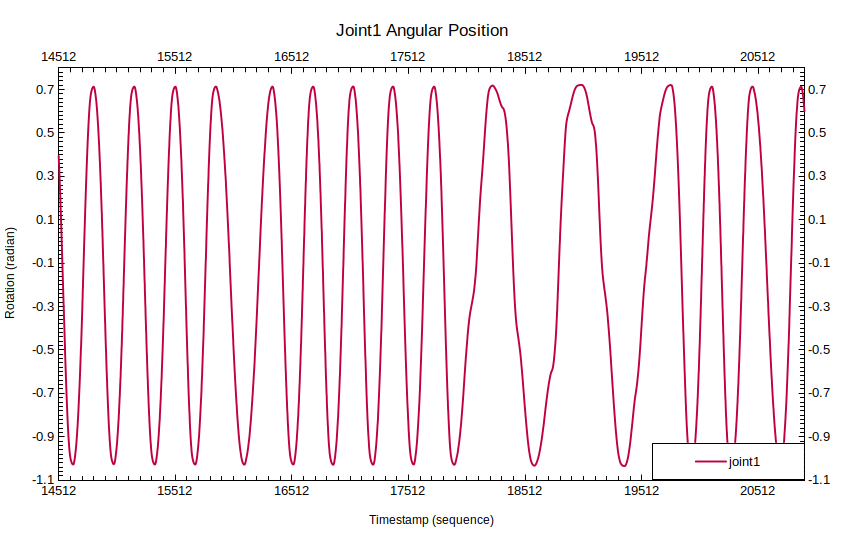
\includegraphics[width=\linewidth]{joint1u.png}
     \caption{}
  \end{subfigure}
  \begin{subfigure}[b]{0.4\linewidth}
    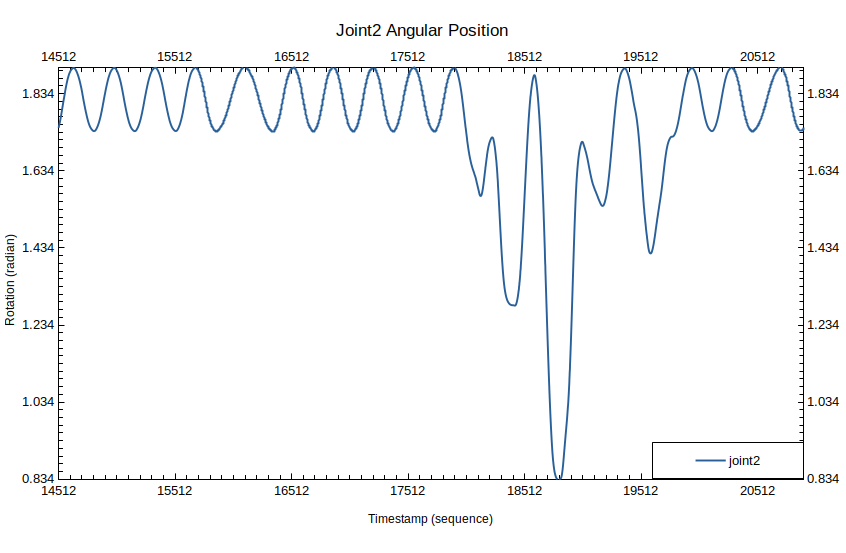
\includegraphics[width=\linewidth]{joint2u.png}
    \caption{}
  \end{subfigure}
  \begin{subfigure}[b]{0.4\linewidth}
    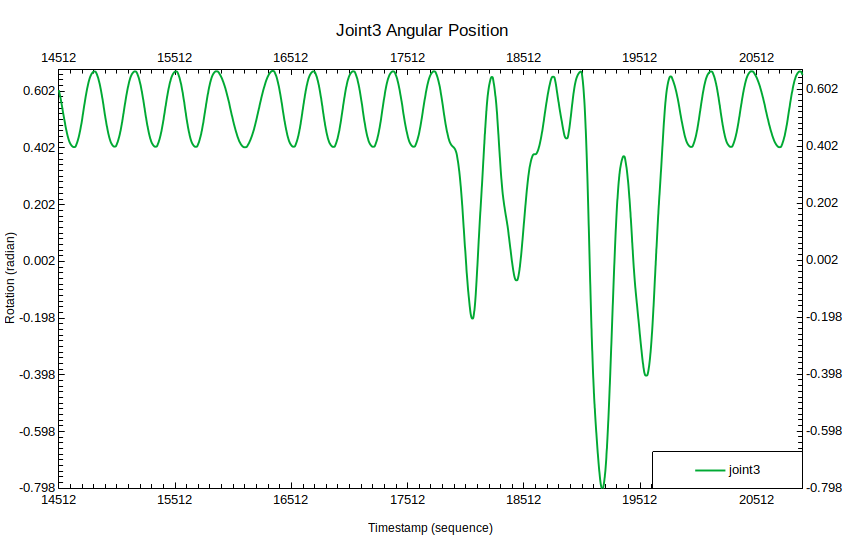
\includegraphics[width=\linewidth]{joint3u.png}
    \caption{}
  \end{subfigure}
  \begin{subfigure}[b]{0.4\linewidth}
    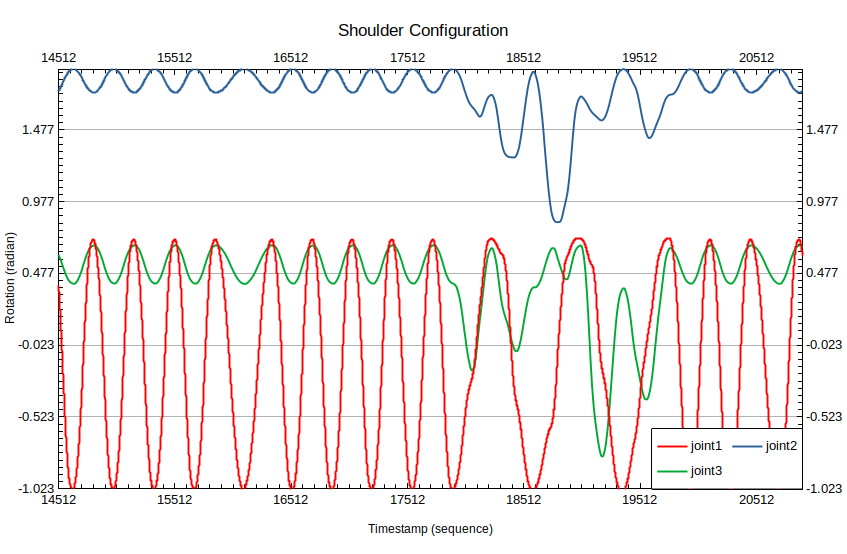
\includegraphics[width=\linewidth]{joint123u.png}
    \caption{}
  \end{subfigure}

  \caption{Reaction from joint1, joint2, and joint3 shows that the planner
   together with the cycle space behave reactively towards the moving object. No rapid movement or rate on the last three joints on \rimini}
  \label{fig:reaction_joint}
\end{figure}`
